The global model was used to infer the electric field, electron densities, and
electron temperatures in the \acs{rpnd} from the metastable measurements.
However, as was described in the development of the model, it is also capable of
predicting the densities of other excited states and the optical emissions of
the \acs{rpnd}. This chapter will describe the measurement of the optical
emissions of the \acs{rpnd} and then the use of these measurements to determine
the \acs{rpnd} wave velocity and electrons temperatures. Finally, the electron
temperatures and the spectral trends will be compared to those obtained from the
global model.

\section{Emission Measurements}

Emissions spectroscopy was conducted at the same operating conditions as the
metastable measurements. Light collection was accomplished with a 1 cm diameter
bundle of optical fibers, butted against the outside of the glass envelope. The
other end was placed at the entrance slit of a ISA Jobin-Yvon SPEX HR460
monochromator. A grating with 1200 grooves/mm was installed in the
monochromator. The entrance slit width was set to 250 $\mu$m and the exit slit
was set at 500 $\mu$m. This was done so as to collect the integrated intensity
of each spectral line.

A photomultiplier tube (\acs{pmt}) of model C31034 was used to record the
changes in intensity over time. The tube voltage was set to 1900 V and was
terminated into a 50 $\Omega$ resistor. Specifications could not be found for
the tube, however measurements demonstrated a rise time of, at most, 3.5 ns.
Unlike the laser-absorption spectroscopy measurements, each emission curve was
averaged over 1000 acquisitions and 5 $\mu$s. Otherwise, the acquisition
settings remained the same.

The range of spectral sensitivity for the photocathode of the \acs{pmt} limited
measurements to transitions occurring between 350-750 nm. The list of observable
transitions is recorded in table~\ref{tbl:transitions}.
\begin{table}
  \centering
  \caption{Table of the observed optical transitions and their transition
    rates.}
  \begin{tabular}{lllll}
    \toprule                                                                    \\
    Initial      & Final        & Wavelength &              &                   \\
    State        & State        & (nm)       & A (s$^{-1}$) & $\sum$A (s$^{-1}$)\\
    \midrule                                                                    \\
    3$^3$P$\odd$ & 2$^3$S       & 388.97     & $9.46\EE6$   & $1.06\EE7$        \\
    4$^1$P$\odd$ & 2$^1$S       & 396.59     & $6.95\EE6$   & $2.52\EE8$        \\
   %5$^3$D       & 2$^3$P$\odd$ & 402.73     & $1.16\EE7$   & $1.64\EE7$        \\
    4$^3$D       & 2$^3$P$\odd$ & 447.28     & $2.46\EE7$   & $3.12\EE7$        \\
    4$^3$S       & 2$^3$P$\odd$ & 471.45     & $9.52\EE6$   & $1.60\EE7$        \\
    4$^1$D       & 2$^1$P$\odd$ & 492.33     & $1.99\EE7$   & $2.70\EE7$        \\
    3$^1$P$\odd$ & 2$^1$S       & 501.71     & $1.34\EE7$   & $5.80\EE8$        \\
    3$^3$D       & 2$^3$P$\odd$ & 587.73     & $7.07\EE7$   & $7.07\EE7$        \\
    3$^1$D       & 2$^1$P$\odd$ & 668.00     & $6.37\EE7$   & $6.37\EE7$        \\
    3$^3$S       & 2$^3$P$\odd$ & 706.72     & $2.79\EE7$   & $2.79\EE7$        \\
    3$^1$S       & 2$^1$P$\odd$ & 728.34     & $1.83\EE7$   & $1.83\EE7$        \\
  \end{tabular}
  \label{tbl:transitions}
\end{table}
Several factors, including the fiber, monochromator grating, and the
photocathode coating resulted in a nonuniform response with wavelength. This was
compensated for with spectral measurements of an Optronic Laboratories M-1179
spectral irradiance standard, powered by an Optronic Laboratories OL 65 power
supply. 

\section{Wave Velocities}

In the analysis of \acs{fiw} discharges, one of the most common means of
comparison is the use of wave velocities. In the studies reported by Vasilyak
\cite{Vasilyak1994}, the velocities were measured using several approaches. In
one, capacitive probes were placed in contact with the dielectric of the
discharge tube, and the time delay between the voltage signals was used as the
wave velocity. In some cases an intensified \acs{ccd} was used to track the
propagation of the wave. Alternately, a photomultiplier tube was positioned
against the dielectric at varying axial locations. This is the approach used
here.

The maximum detectable velocity was limited by several factors. Data were only
available at intervals of 1 ns. As the maximum separation of measurement
locations was 15.24 cm, this set an upper limit of about 1.5$\times10^8$ m/s.
Additional limitations were imposed by the jitter of the pulser output. Overall,
the maximum detectable wave velocity was $5.0\times10^7$ m/s.

The velocities were determined as an average of the all the emission curves
recorded. In each case, the curve at each axial location was interpolated with a
smoothing spline. The time of the maximum derivate of the emission curves was
used as the reference point in each case. The distance between the measurement
locations was then divided by the time delay between the maximum derivatives.
The results of these calculations are recorded in table~\ref{tbl:velocities}.
\begin{table}
  \centering
  \caption{Wave velocities in the \acs{rpnd}.}
  \label{tbl:velocities}
  \begin{tabular}{lll}
    \toprule                                                      \\
    Pressure  & Upstream                & Downstream              \\
    (Torr)    & Velocity (m/s)          & Velocity (m/s)          \\
    \midrule                                                      \\
    8.0       & $3.01\pm1.21\times10^7$ & $1.73\pm0.26\times10^7$ \\
    16.0      & $1.46\pm0.19\times10^7$ & $6.80\pm1.75\times10^6$ \\
  \end{tabular}
\end{table}

Delays in the emissions at the different axial locations only appeared for the
8.0 and 16.0 Torr conditions. The propagation of the discharge across the
chamber was essentially instantaneous for all other conditions. Vasilyak et al.\
note that it is difficult to compare the velocities of \acs{fiw} discharges as a
result of numerous dependencies and poorly understood physics. In the \acs{fiw},
the velocity varies with pressure, gas, outer dielectric, pulse voltage, and
preionization. There is no reason to suspect that the situation is any different
for the \acs{rpnd}. That said, the measured values fall within the wide range
that has previously been associated with streamers, \acs{fiw}s, and \acs{rpnd}s.

The early work of Schonland and Collens \cite{Schonland1933} determined that the
luminous front of lightning propagated with a velocity of $0.72-5.3\times10^7$
m/s for the forward and return stroke. The studies reported by Vasilyak et al.
\cite{Vasilyak1994} give a range of approximately $2-5\times10^7$ m/s for a 200
kV \acs{fiw} in helium at pressures from 0.1-760 Torr. Propagation velocities
for atmospheric plasma jets of helium have been measure at about $10^5$ m/s
\cite{Lu2006} with simulations providing confirmation \cite{Naidis2010} of these
values. Fast imaging by Ito et al. \cite{Ito2010} determined a velocity of
$10^6$ m/s for a hydrogen \acs{rpnd}.


\section{Electron Temperatures}

Measurement of the electron temperature in \acs{rpnd}s poses a large difficulty
for several reasons. The most significant of which is the concept of temperature
itself. As was noted in Chapter~\ref{chp:modeling}, the \acs{rpnd} is a highly
dynamic system which does not necessarily result in a population of electrons
with a Maxwell-Boltzmann distribution. In the absence of this property, the
``temperature'' quantity can have an ambiguous meaning. Often, the reported
temperature describes the Maxwell-Boltzmann distribution which best matches
measured some choice of plasma properties (such as plasma emissions). In other
cases, the temperature may describe the mean electron energy of the \acs{eedf},
such as in Chapter~\ref{chp:modeling} or in the work of Starikovskaia and
Starikovskii \cite{Starikovskaia2001}.

The temperatures generated in these two cases will coincide only for a limited
number of situations and the choice of diagnostics. Thus, it is of interest to
search for useful electron temperature diagnostics which apply to the
\acs{rpnd}. The electron temperature of a system is most often determined by the
use of electrostatic probes, such as those discussed by Lieberman
\cite{Lieberman2005}. However, as was discussed at the beginning of
Chapter~\ref{chp:metastables}, physical probes are not a reasonable option of
the \acs{rpnd}. An active optical technique, such as Thomson scattering
\cite{VanGessel2012}, would be an ideal solution if the electron densities in
the \acs{rpnd} were not below its sensitivity threshold.

Therefore, several attempts were made to translate the plasma emission
measurements to electron temperatures. Such techniques have been successful in
the analysis of steady-state systems with relatively low electron densities,
however the applicability to very dynamic discharges is not a given and must be
qualified \cite{Kunze2009}. 

\subsection{Boltzmann Plots}

When the population of two excited states are in equilibrium with the electrons,
the ratio of their densities can be written as \cite{Griem2005}
\begin{equation}
  R = \frac{\lambda_{i,j}A_{i,j}g_j}{\lambda_{i',j'}A_{i',j'}g_{j'}}
      \exp\left( -\frac{\Delta\epsilon_{i,j} - \Delta\epsilon_{i',j'}}
                       {\kB T_e} \right),
\end{equation}
where the subscripts represent different electronic states, $\lambda$ is the
transition wavelength, $A$ is the spontaneous transition rate, $g$ is
statistical degeneracy, and $\Delta\epsilon$ is the energy separation between
the identified states. In this case, the line ratios only depend on the electron
temperature and physical quantities that are well-tabulated for helium.

This approach can be applied to several successive transitions by plotting the
quantity
\begin{equation}
  \log\left(\frac{I_{i,j}\lambda_{i,j}}{g_jA_{ij}}\right)
\end{equation}
with respect to $\Delta\epsilon_{i,j}$, where $I$ is the measured intensity of
the optical transition. Ideally, the plotted points would form a line where the
negative reciprocal is equal to the electron temperature. This is most
frequently referred to as a Boltzmann plot. 

The emissions data for the wavelengths recorded in table~\ref{tbl:transitions}
was compiled into a series of intensities for each time step. A Boltzmann plot
was then generated for each time step and a line was fit to the data using a
least-squares algorithm. This produced the temperature estimates seen in
figure~\ref{fig:boltcomp}.
\begin{figure}
  \centering
  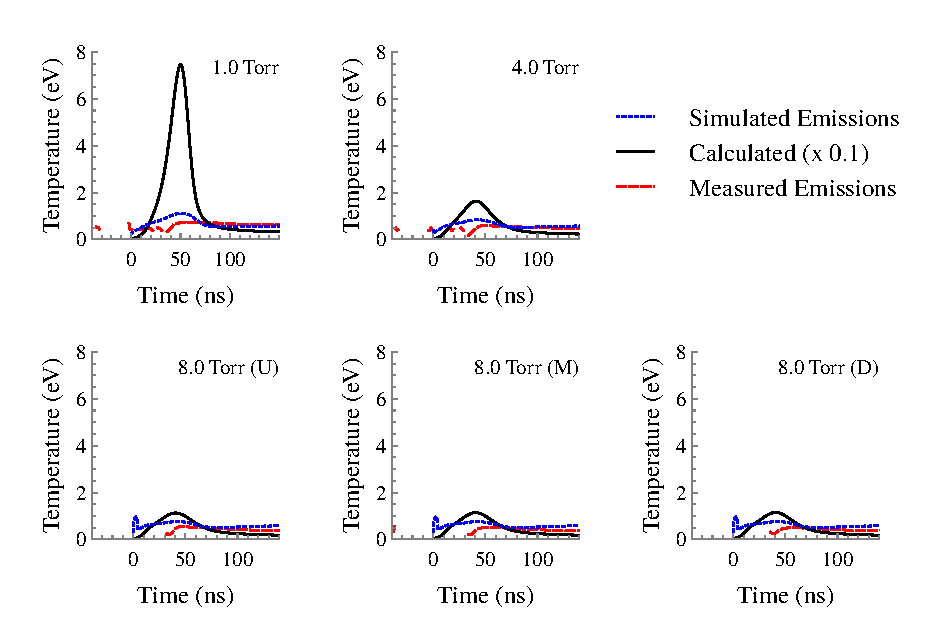
\includegraphics{./chapters/emissions/figures/boltcomp.eps}
  \caption{Temperatures estimated using Boltzmann plots of the measured emissions
    (dashed, red lines) and simulated emissions (dotted, blue lines) compared to
    the simulated temperatures (solid, black line).}
  \label{fig:boltcomp}
\end{figure}
Negligible plasma emissions occurred prior to the pulse, preventing any analysis
during that period of time. Estimates of the electron temperature using the
Boltzmann plot approach proved to provide poor predictions. Peak temperatures
were underestimated by at least a factor of ten, if not more. This disagreement
is not altogether unexpected--the assumption of equilibrium between the excited
states and the electrons is most certainly violated on such short time scales,
simply as a result of the finite time required for electron-atom collisions to
occur. This is confirmed by the poor quality of the temperature estimates
generated from the simulated emissions.

After the pulse, when the electrons are cooling primarily through elastic
collisions, it might be expected that the atomic state populations would relax
to an equilibrium distribution. While this is true for a long enough time
period, this behavior is not observed for the length of time under
consideration. Instead, the non-equilibrium distribution of atomic states that
is established during the pulse lasts well into the afterglow. As Kunze notes,
``one always has to check if indeed the assumption of a Boltzmann distribution
is justified \ldots, equilibrium may not be reached even if the steady-state
conditions seem to indicate that.'' \cite{Kunze2009}

Generally, the Boltzmann plots are poor predictors of the electron temperature
for the time period under consideration. This almost certainly results from the
inapplicability of the Boltzmann distribution to excited state populations. As
can be seen in figure~\ref{fig:boltex},
\begin{figure}
  \centering
  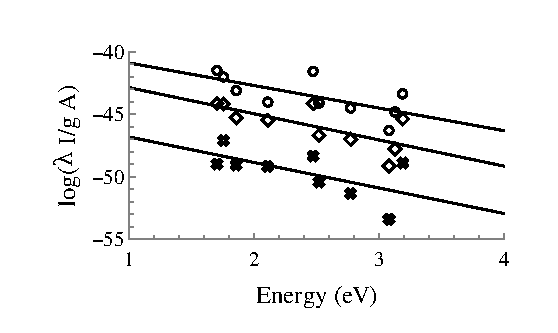
\includegraphics{./chapters/emissions/figures/boltex.eps}
  \caption{Boltzmann plot examples for the \acs{rpnd}}
  \label{fig:boltex}
\end{figure}
the plots show a large deviation from line that would be expected from theory.
To some extent, this too may be indicative of inaccuracies in the line intensity
measurements, however even after removing the transitions with relatively small
signals, no clear lines emerge. 

\subsection{Coronal Model}

In place of the assumption about an equilibrium distribution between excited
states, another approach is the use of the coronal model. In this case, the
states are considered to be excited by electrons, but to decay via optical
transitions. This model excels at low densities where states are not subject to
a great degree of mixing and inter-atomic collisions can be neglected. Again,
these assumptions do not necessarily apply to the \acs{rpnd}.

Per Kunze \cite{Kunze2009}, the line intensity ratio resulting from the coronal
model may be expressed as
\begin{equation}
  R = \frac{\lambda_{i',j'}A_{i,j}\sum A_{i'} K_{0,i}(T_e)}
  {\lambda_{i,j}A_{i',j'}\sum A_{i} K_{0,i'}(T_e)}
\end{equation}
where the sum is over all possible radiative decay pathways, the subscript `0'
is the ground state, and $K$ is the rate coefficient. Note that the rate
coefficients are explicitly functions of the electron temperature. The upper
states used for this line ratio must be carefully chosen so as to limit
sensitivity to collisional mixing of excited states. Likewise, the rate
coefficient ratio should exhibit a monotonic trend with electron temperatures.

Several ratios have been suggested by Kunze and others, including:
4$^3$S-2$^3$P$\odd$ over 4$^1$S-2$^1$P$\odd$, 3$^3$S-2$^3$P$\odd$ over
3$^1$S-2$^1$P$\odd$, and 4$^3$S-2$^3$P$\odd$ over 4$^1$D-2$^1$P$\odd$. The
ratios with the upper state in an S subshell are attractive as they are less
susceptible to collisional mixing between states of equal $n$ \cite{Kunze2009}.
Limited emission intensity prevented accurate measurements of the
4$^1$S-2$^1$P$\odd$ transition. As a result, only the former two ratios were
considered for analysis.

Like the other mentioned ratios, 4$^3$S-2$^3$P$\odd$ over 4$^1$D-2$^1$P$\odd$
compares a transition from the triplet manifold to one from the singlet
manifold. Triplet-singlet ratios have been found to be mostly dependent to
electron temperature which makes them ideal for this purpose \cite{Griem2005}.
Figure~\ref{fig:conversion}
\begin{figure}
  \centering
  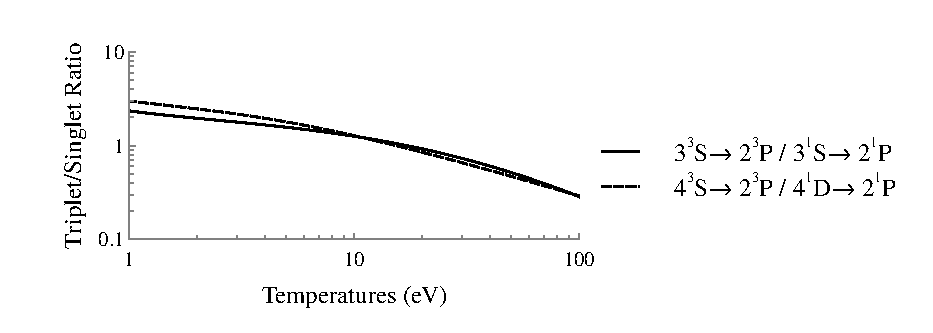
\includegraphics{./chapters/emissions/figures/conversion.eps}
  \caption{The emission ratios of 4$^3$S-2$^3$P$\odd$ over 4$^1$D-2$^1$P$\odd$ 
    and 3$^3$S-2$^3$P$\odd$ over 3$^1$S-2$^1$P$\odd$, as functions of the
    electron temperature.}
  \label{fig:conversion}
\end{figure}
shows the relation between the emission intensity of the two transitions and the
electron temperature of the system. The rate coefficients were calculated with
the assumption of a Maxwell-Boltzmann distribution, using the cross sections
produced by Ralchenko et al. \cite{Ralchenko2008}. Though it is possible to
convert the measured and simulated line ratios to temperatures using these
results, they may not necessarily correlate to the actual temperatures of the
system.

The calculated conversion between triplet-singlet ratio was used to estimate the
temperature of the \acs{rpnd} experiment in addition to the simulated emissions.
The results can be found in figure~\ref{fig:rat2comp}.
\begin{figure}
  \centering
  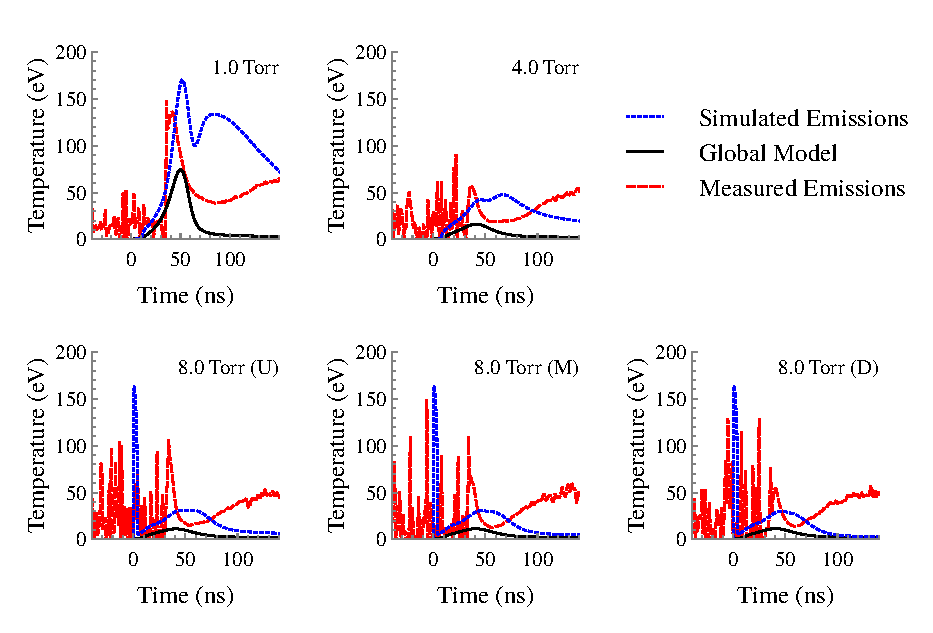
\includegraphics{./chapters/emissions/figures/rat2comp.eps}
  \caption{Estimates of the electron temperatures based on the ratio of the
    4$^3$S-2$^3$P$\odd$ and 4$^1$D-2$^1$P$\odd$ transitions. The estimates were
    generated for the simulated emissions (dotted, blue lines) and measured
    emissions (dashed, red lines), and are compared to the actual temperature
    results from the global model simulation (solid, black lines).}
  \label{fig:rat2comp}
\end{figure}
Generally, neither the simulated or measured ratios provided a good estimate of
the electron temperatures. Unlike the Boltzmann plots, both tended to
overestimate the temperature of the \acs{rpnd}. As the higher temperatures
relate to a lower triplet-singlet ratio, this suggests either an excess in
4$^1$D states, or a deficit of 4$^3$S states. Additionally, both the measured
and simulated ratios show growing or otherwise elevated temperature well after
the pulse. This might be a consequence of the collisional mixing described by
Kunze. Also notable is the disagreement between the measured and simulated
ratios. For several periods of time the trends are entirely opposite. Similar
issues were recorded by Boivin et al. \cite{Boivin2007} who suggested that
improved data for the $n=5$ transitions may lead to better agreement.

As suggested above, the ratio of 3$^3$S-2$^3$P$\odd$ to 3$^1$S-2$^1$P$\odd$, may
offer a better means by which to measure the electron temperature. The greater
energy spacing between states of equal $n$ promises to reduce collisional
mixing. Likewise, both of the upper states are from the S subshell, as
recommended by Kunze \cite{Kunze2009}. The promise of this approach is
immediately apparent in figure~\ref{fig:rat1comp}.
\begin{figure}
  \centering
  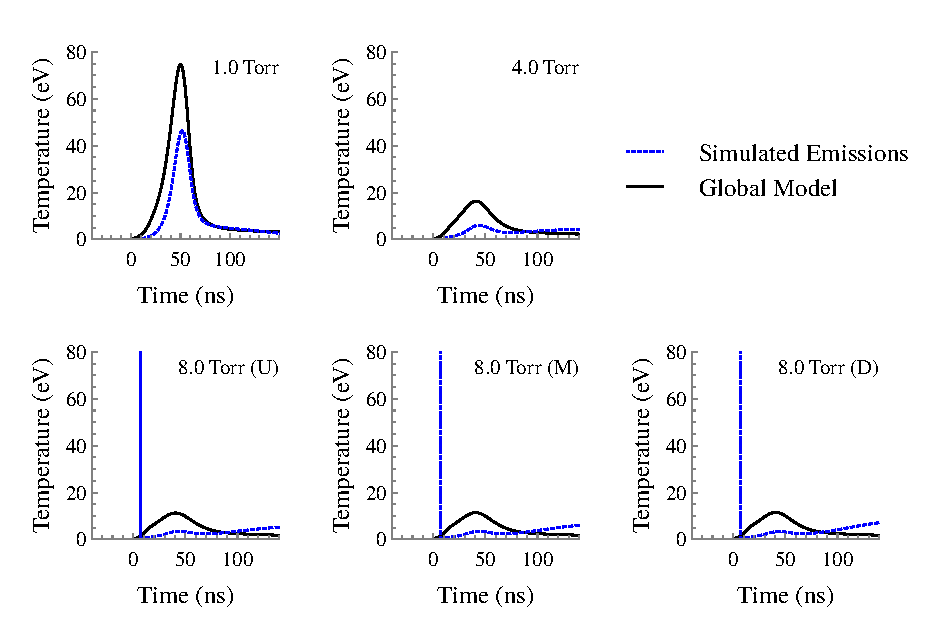
\includegraphics{./chapters/emissions/figures/rat1comp.eps}
  \caption{Estimates of the electron temperatures based on the ratio of the
    3$^3$S-2$^3$P$\odd$ to 3$^1$S-2$^1$P$\odd$, transitions. The estimates were
    generated for the simulated emissions (dotted, blue lines) and measured
    emissions (dashed, red lines), and are compared to the actual temperature
    results from the global model simulation (solid, black lines).}
  \label{fig:rat1comp}
\end{figure}
The temperature estimates based on the simulated emissions show excellent
agreement with the temperatures from the global model. This is true both in
terms of the magnitude of the values and the overall behavior of the trends.
The initial increase in temperature is captured particularly well, with only
moderate deviations in the afterglow. The differences in the afterglow are
likely the result of the radiative cascade which occurs soon after the pulse
ends. In this process, the relaxation of the higher excited states serves to
boost the density of the lower states.

In contrast, the experimental results differ vastly from the other two
temperature trends. In part, this can be attributed to the experimental
difficulties. The two lines, both in wavelengths approaching the infrared, are
not well converted into electrons by the photocathode of the \acs{pmt}. As a
result, the absolute intensities of these lines were particularly low, leading
to a significant amount of uncertainty. That said, the 4.0 Torr operating
condition exhibited sufficient intensities for both lines for temperature
estimates to be made during and after the pulse. In contrast to the temperature
from the global model, the emission measurements suggest that the temperature
peaks at 4.9 eV followed by a rapid relaxation to about 0.5 eV.

Given the low intensities, difficulty in obtaining accurate intensity
measurements \cite{Griem2005}, and the sensitivity of the temperature estimate
to the line ratio, these results should be considered quite preliminary. The use
of these transitions is promising for measurements of the electron temperature
in the \acs{rpnd}--the global model simulations show a good agreement between
the estimates and the actual temperatures, and the ratio changes quickly enough
to capture at least some of the \acs{rpnd} dynamics. This measurement could be
improved by the used of a photocathode with improved response to this spectral
region and selection of a monochromator grating with better efficiency for these
lines.

\section{Global Model Comparison}

In light of the disagreement between the measured and simulated line ratios, it
is informative to consider a comparison of the measured emission trends to the
simulated emission trends. This process can help to identify additional
processes, issues with the rate constants or cross sections, and features
resulting from non-Maxwellian \acs{eedf}s.

\section{Summary}
